% Asset ID: FA21InequalitiesTikZ-002
% Source: FP1 PDF Ex 4A + teacher transcript
% Related lesson section: Section 9; Worked Example 2
% Purpose: Sign sketch for (x-2)(x+2)<0.
% Boundary status: Internal portal enrichment, not official CCEA Further Mathematics specification content.
\documentclass[tikz,border=8pt]{standalone}
\usepackage{amsmath}
\usepackage{xcolor}
\definecolor{Canvas}{HTML}{FAF9F6}
\definecolor{Ink}{HTML}{2C2C2E}
\definecolor{LineSoft}{HTML}{E5E5EA}
\definecolor{Gold}{HTML}{C5A059}
\definecolor{WarmPink}{HTML}{FBEFEF}
\begin{document}

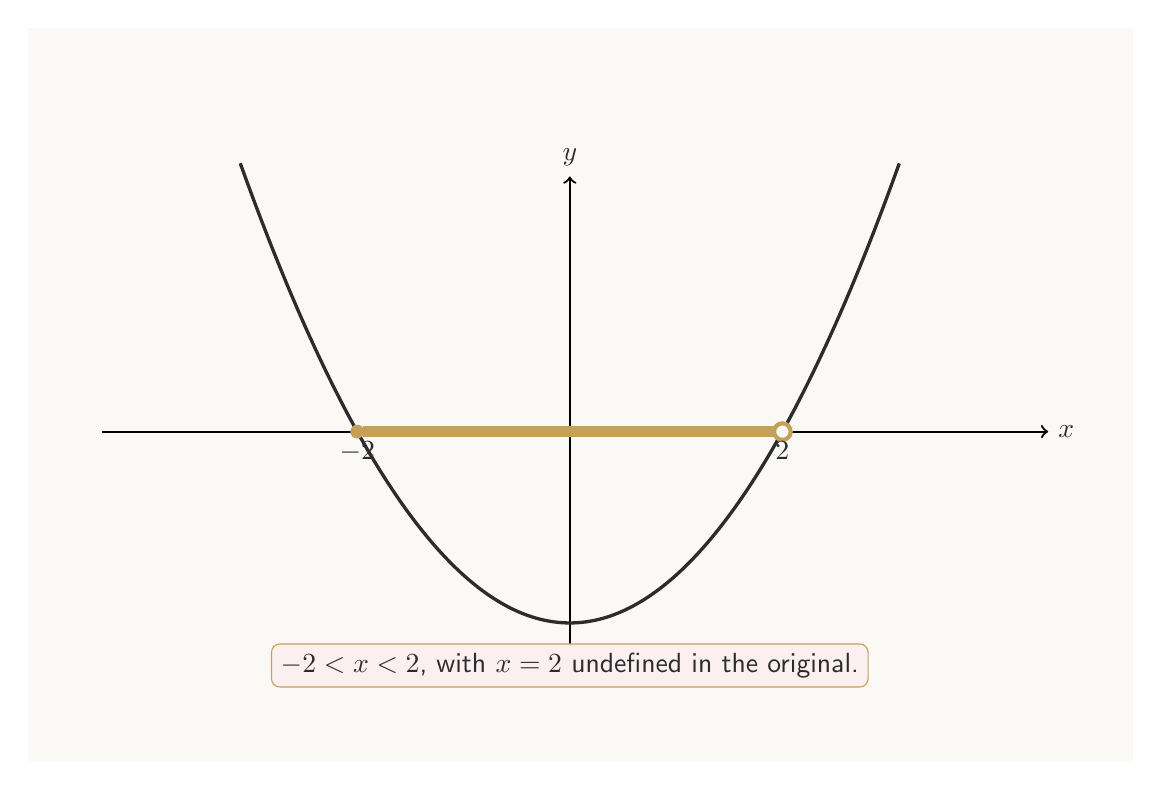
\begin{tikzpicture}[x=1.35cm,y=1.35cm,every node/.style={font=\sffamily,text=Ink}]
\fill[Canvas] (-5.1,-3.1) rectangle (5.3,3.8);
\draw[->,thick] (-4.4,0)--(4.5,0) node[right] {$x$};
\draw[->,thick] (0,-2.3)--(0,2.4) node[above] {$y$};
\draw[Ink,very thick,domain=-3.1:3.1,samples=100,smooth] plot (\x,{0.45*(\x*\x-4)});
\draw[Gold,line width=4pt] (-1.95,0)--(1.95,0);
\fill[Gold] (-2,0) circle (2.5pt);\draw[fill=Canvas,draw=Gold,line width=1.5pt] (2,0) circle (3pt);
\node[below] at (-2,0) {$-2$};\node[below] at (2,0) {$2$};
\node[fill=WarmPink,draw=Gold,rounded corners=3pt] at (0,-2.2) {$-2<x<2$, with $x=2$ undefined in the original.};
\end{tikzpicture}

\end{document}
